\documentclass[a4paper]{article}        % Standaard een kolom layout
\usepackage[english]{babel}               % Stel woordafbrekingen en referentienamen in
\usepackage{graphicx}                   % Afbeeldingen weergeven
\usepackage{float}                      % Figuren op plaats waar ze gedefinieerd staan: [H]
\usepackage{lmodern}                    % Gebruik modern lettertype
\usepackage[T1]{fontenc}
\usepackage[hidelinks]{hyperref}        % Referenties aanklikbaar in PDF, geen kaders rond weergeven
\usepackage[margin=1.5in]{geometry}
\usepackage[binary-units,per-mode=symbol]{siunitx}                    % SI unit symbolen
\usepackage{amsmath}                    % Matrices en vergelijkingen
\usepackage{subcaption}                 % Subfiguren
\usepackage{tabularx}
\usepackage[parfill]{parskip}
\DeclareSIUnit\dbm{\decibel{}m}         % Voeg dBm toe als eenheid
\usepackage{tikz}
\usetikzlibrary{shapes,arrows}
\usepackage{csvsimple}
\usepackage{hyperref}
\usepackage{natbib}


\title{High Frequency Design: \\ Design of an RF front-end for a GPS receiver}
\author{Thomas Deckmyn}
\date{\today}
\begin{document}
\maketitle

\section{Introduction}
\section{Circuit Design}
	\subsection{LNA}

	\textbf{Misschien specificaties nog eens oplijsten?}\\\\
	The design of the LNA first requires a choice of topology. A common emittor toplogy is the best choice in this case, because it yields the highest power gain and has a moderate input and output impedance, hence it can easily be matched to a $\SI{50}{\ohm}$ system.
		\subsubsection{DC Operating Point}
			When determining the DC operating point for the BFP740 transistor a trade-off has to be made between minimal NF and maximum linearity. Based on the characteristics found in the datasheet\cite{transdatasheet} of the transistor we choose $V_{CE} = \SI{4}{\volt}$ and $I_C = \SI{20}{\milli\ampere}$ to obtain the highest possible linearity, i.e. $IP3 = \SI{27}{\dbm} $. For $I_C = \SI{20}{\milli\ampere}$ the NF is $\SI{0.7}{\decibel}$, which still leaves a lot of margin to stay below the specified NF of $\SI{1.5}{\decibel}$. From the datasheet we know that $\beta = 300$, which yields $I_B = \frac{I_C}{\beta} = \SI{66}{\micro\ampere}$, hence the circuit shown in Figure \ref{fig:lna_ce} can be constructed. DC blocking capacitor are added as not to interrupt the DC operating point of the transistor. The DC feed ensures DC current where needed and prevents RF current from entering the DC voltage source. \\

			\begin{figure}[H]
			\centering
				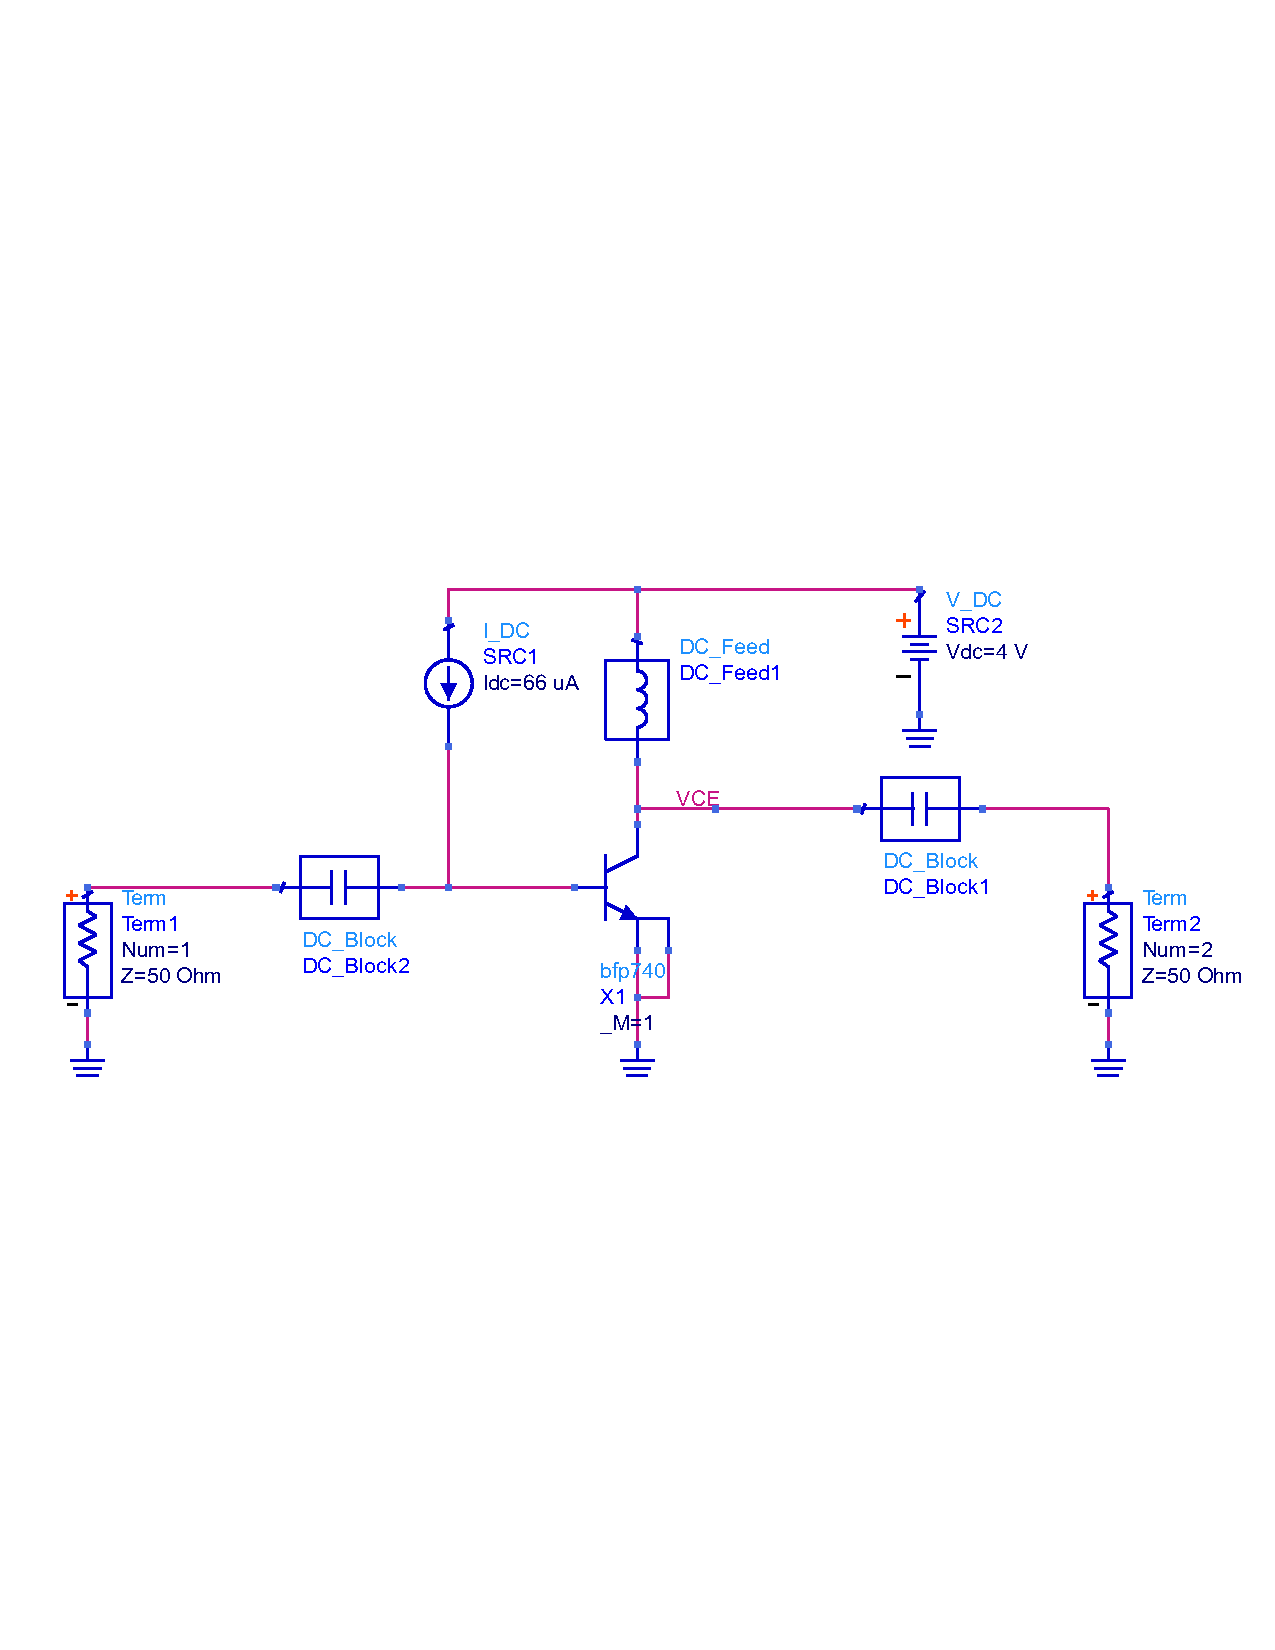
\includegraphics[width=0.8\textwidth]{fig/LNA/LNA_start.pdf}
			\caption{Common emitter topology}
			\label{fig:lna_ce}
			\end{figure}

			To enable the $\SI{5}{\volt}$ supply the DC feed can be replaced by a resistor, which will lower the collecor emittor voltage. We want $I_C$ to still be $\SI{20}{\milli\ampere}$ and $V_{CE}$ $\SI{4}{\volt}$. This means we need a $\SI{1}{\volt}$ voltage drop over the resistor and $\SI{20}{\milli\ampere}$ going through it, hence $R = \frac{V}{I} = \SI{50}{\ohm}$. We obtain the circuit in Figure \ref{fig:lna_5V}.

			\begin{figure}[H]
			\centering
				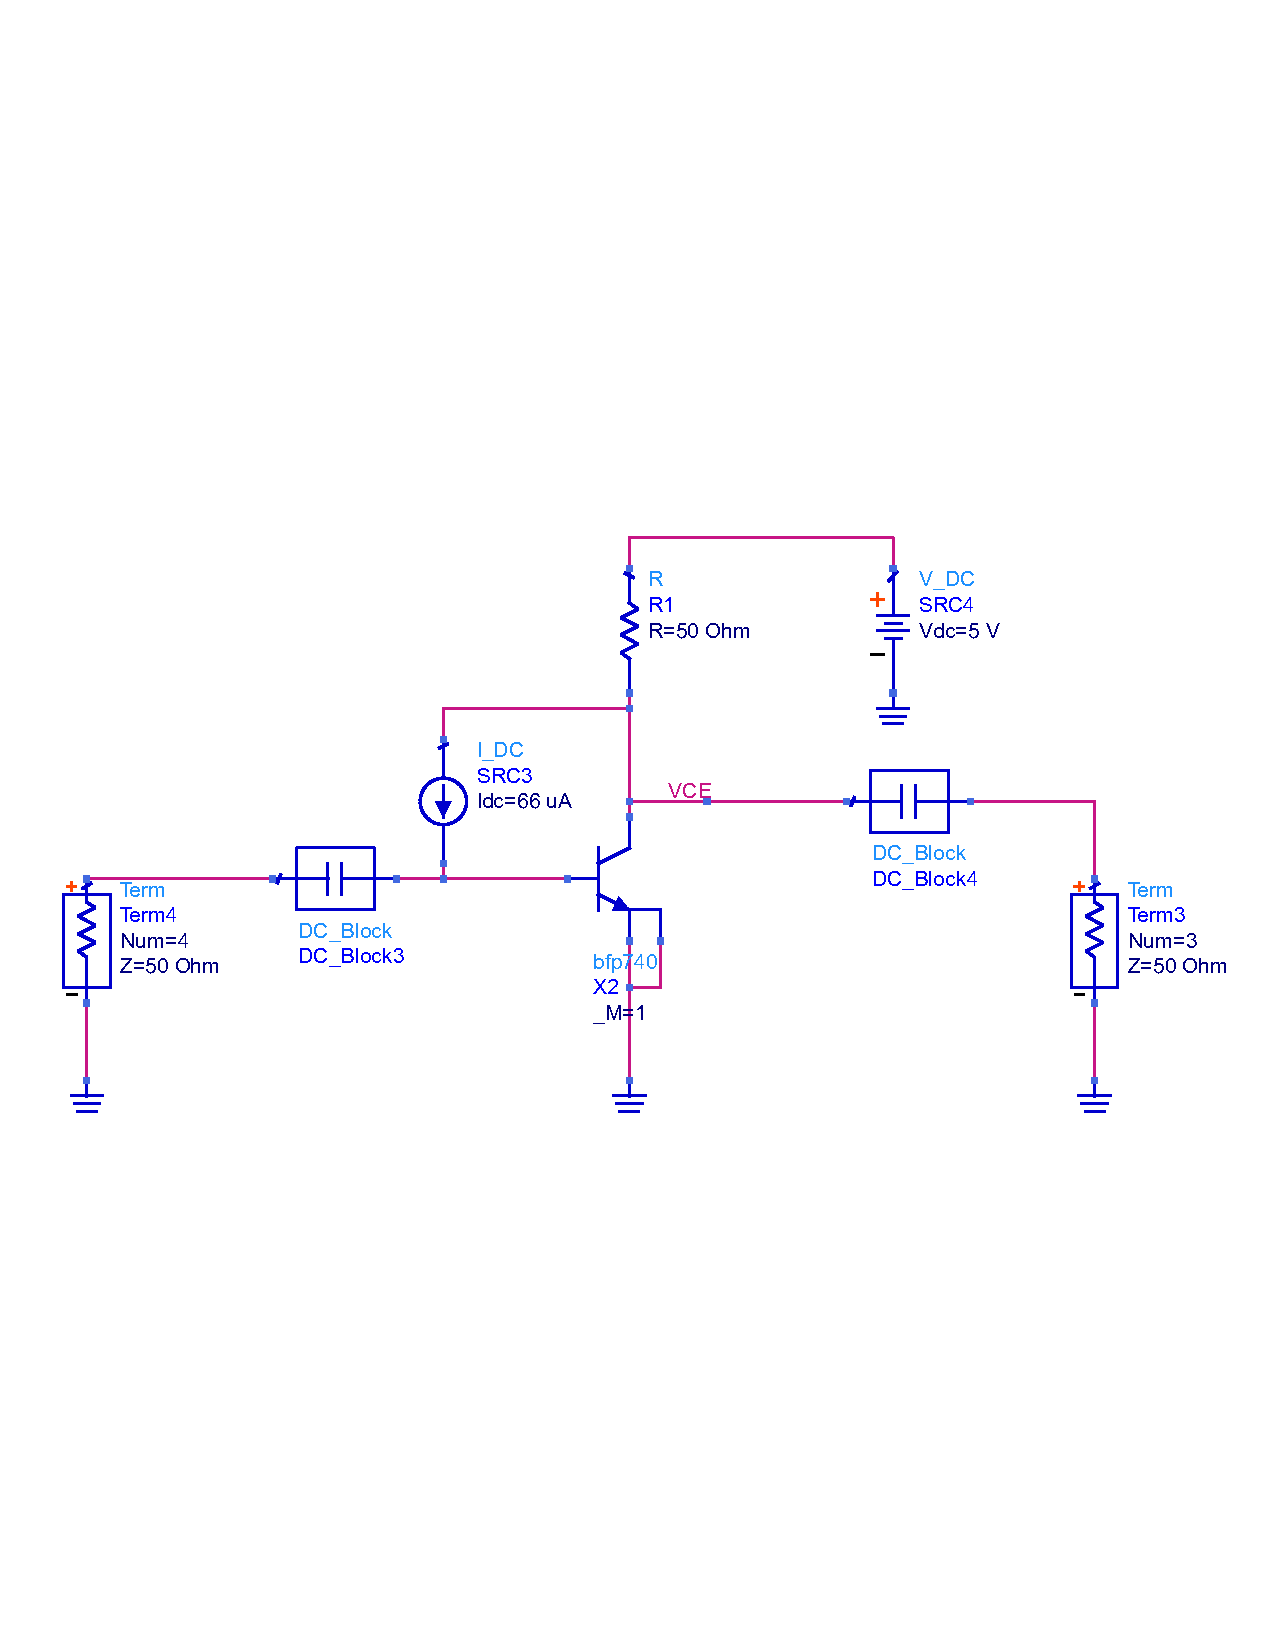
\includegraphics[width=0.8\textwidth]{fig/LNA/LNA_5V.pdf}
			\caption{DC feed replaced with resistor enabling 5V supply}
			\label{fig:lna_5V}
			\end{figure}

		\subsubsection{Stability}
			To decide wether the amplifier is stable, we draw the input and output stability circles. We know that in the center of the Smith Chart $\Gamma_{in} = |S_{11}] < 1$ and $\Gamma_{out} = |S_{22}| < 1$, hence if the stability circles do not intersect with the unity circle the amplifier is stable for all possible passive terminations at the design frequency.\cite{pozar} The value of the stability resistor(s) tunes diameter and position of the stability circle, hence stability can be obtained by tuning the resistor(s).\\

			 To obtain a stable amplifier there a few choices that can be made concerning the position of the stability resistor, i.e. shunt or series at input or output, or a combination of multiple resistors. As we are designing a low noise amplifier a series resistor at the input would be a bad choice, as this would increase the NF considerably. To stabilize the amplifier with solely a shunt resistance at the input a very high resistance is needed (order of $\SI{100}{\kilo\ohm}$), which would put non realisable constraints on the matching network. After analyzing the two remaining options and combinations, we conclude that best performance with respect to NF and gain is achieved with a series resistance at the output and a shunt resistance at the input. The realized stabilization circuit can be seen in Figure \ref{fig:lna_stable}.

			 \begin{figure}[H]
				\centering
				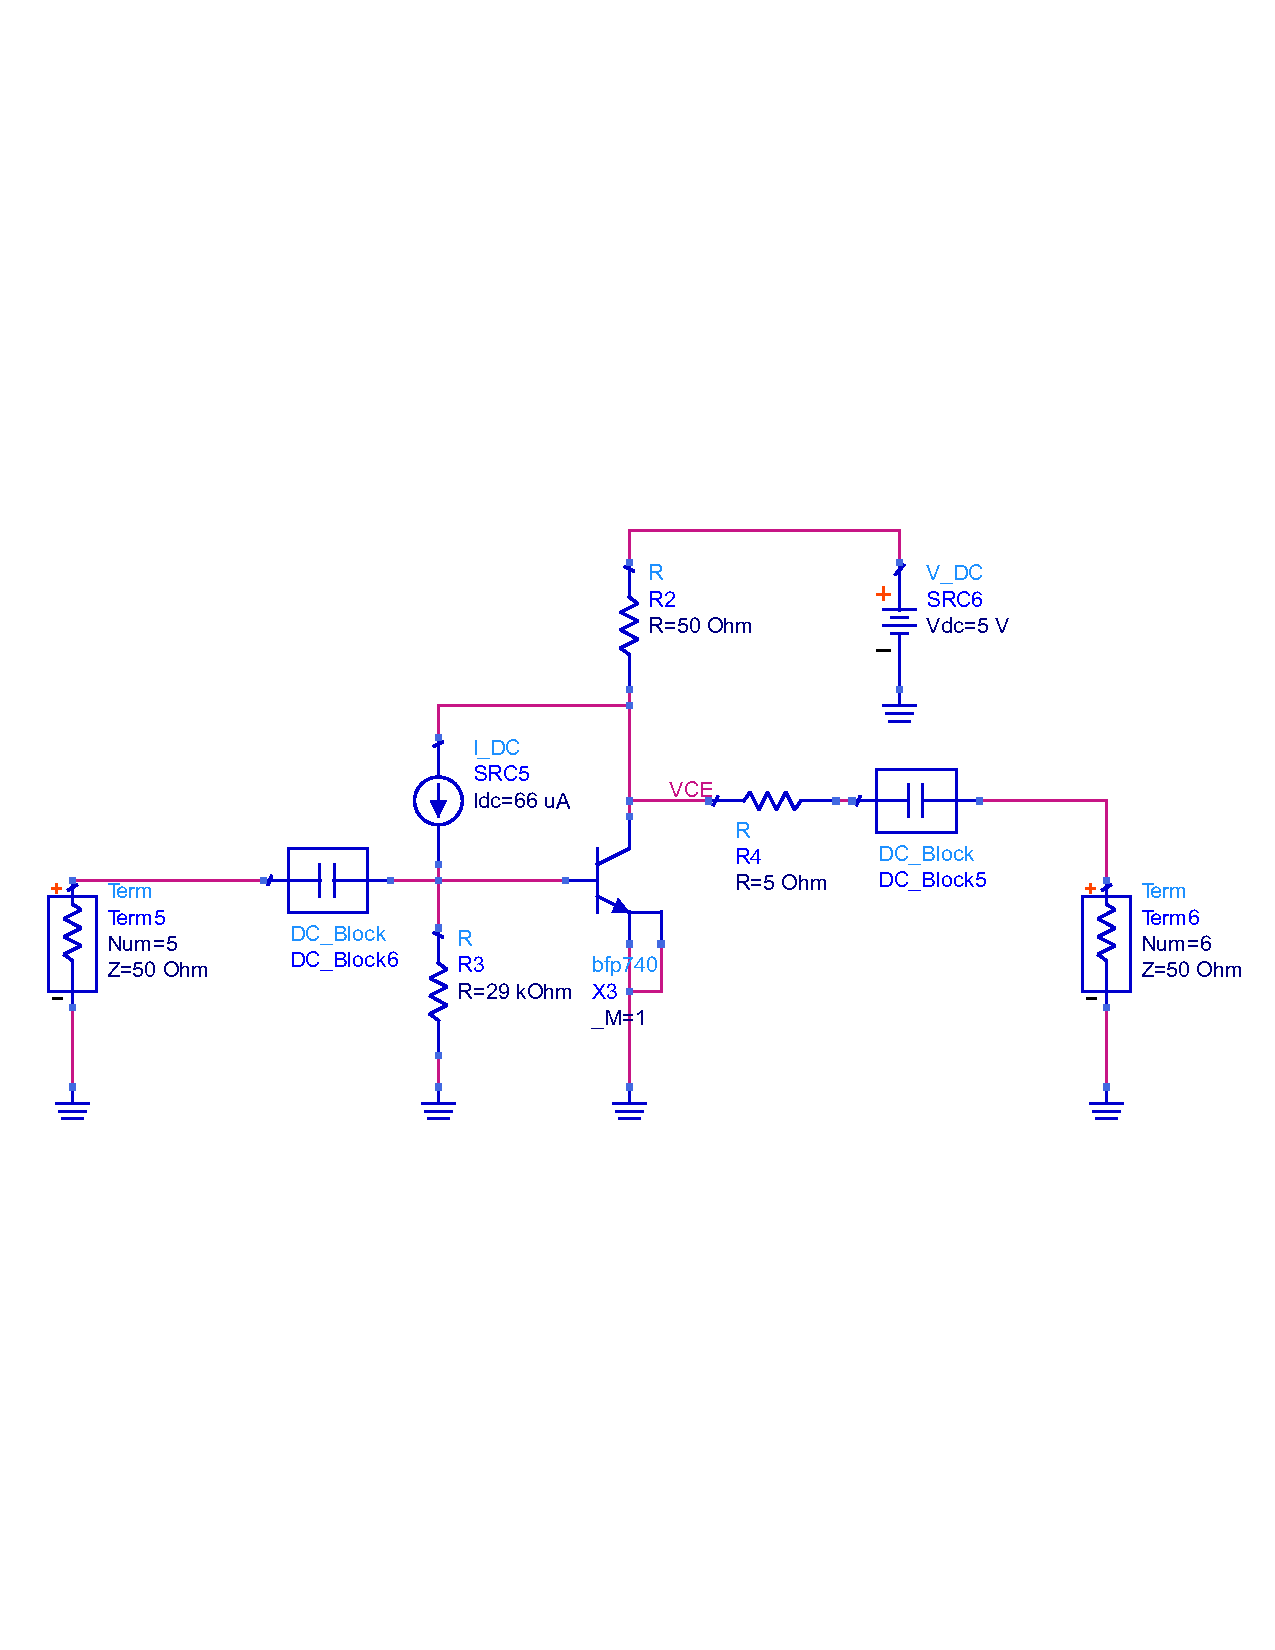
\includegraphics[width=0.8\textwidth]{fig/LNA/LNA_stable.pdf}
				\caption{Circuit for LNA with added stabilization resistors}
				\label{fig:lna_stable}
			\end{figure}

		\subsubsection{Gain and Noise Matching and Biasing}
		\label{sec:lna_matching}

			What is still left to do is selecting the load and source reflection coefficients. For this we draw constant gain circles in the output plane and constant noise circles in the input plane. Next, we choose the load reflection coefficient $\Gamma_L$ in such a way that the source reflection coefficient $\Gamma_S$ is within the constant noise circle of $\SI{1.5}{\decibel}$ as specified. To achieve a NF that is below $\SI{1.5}{\decibel}$ we will need to sacrifice gain at the output, as can be seen in Figure \ref{fig:lna_circles}. The load reflection $\Gamma_L$ is chosen on the $\SI{20}{\decibel}$ gain circle and then the source reflection $\Gamma_S$ is within the $\SI{1.5}{\decibel}$ noise circle. \\

			First, the output is matched such that $\Gamma_L$ is located at $Z_0 (0.645 + j 0.109)$ on the Smith Chart, which will reduce the gain to $\SI{20}{\decibel}$, but the NF will be within the specifications. Second, the input impedance is matched to $\SI{50}{\ohm}$. The matching is performed using the Smith Chart Tool in ADS and both networks consist of a piece of transmission line and a capacitor. The circuit with the added matching networks is shown in Figure \ref{fig:lna_pre_layout}. The DC blocks can be omitted as the capacitors of the matching network now act as DC blocks. 

			\begin{figure}[H]
			\begin{subfigure}{0.5\textwidth}
				\centering
				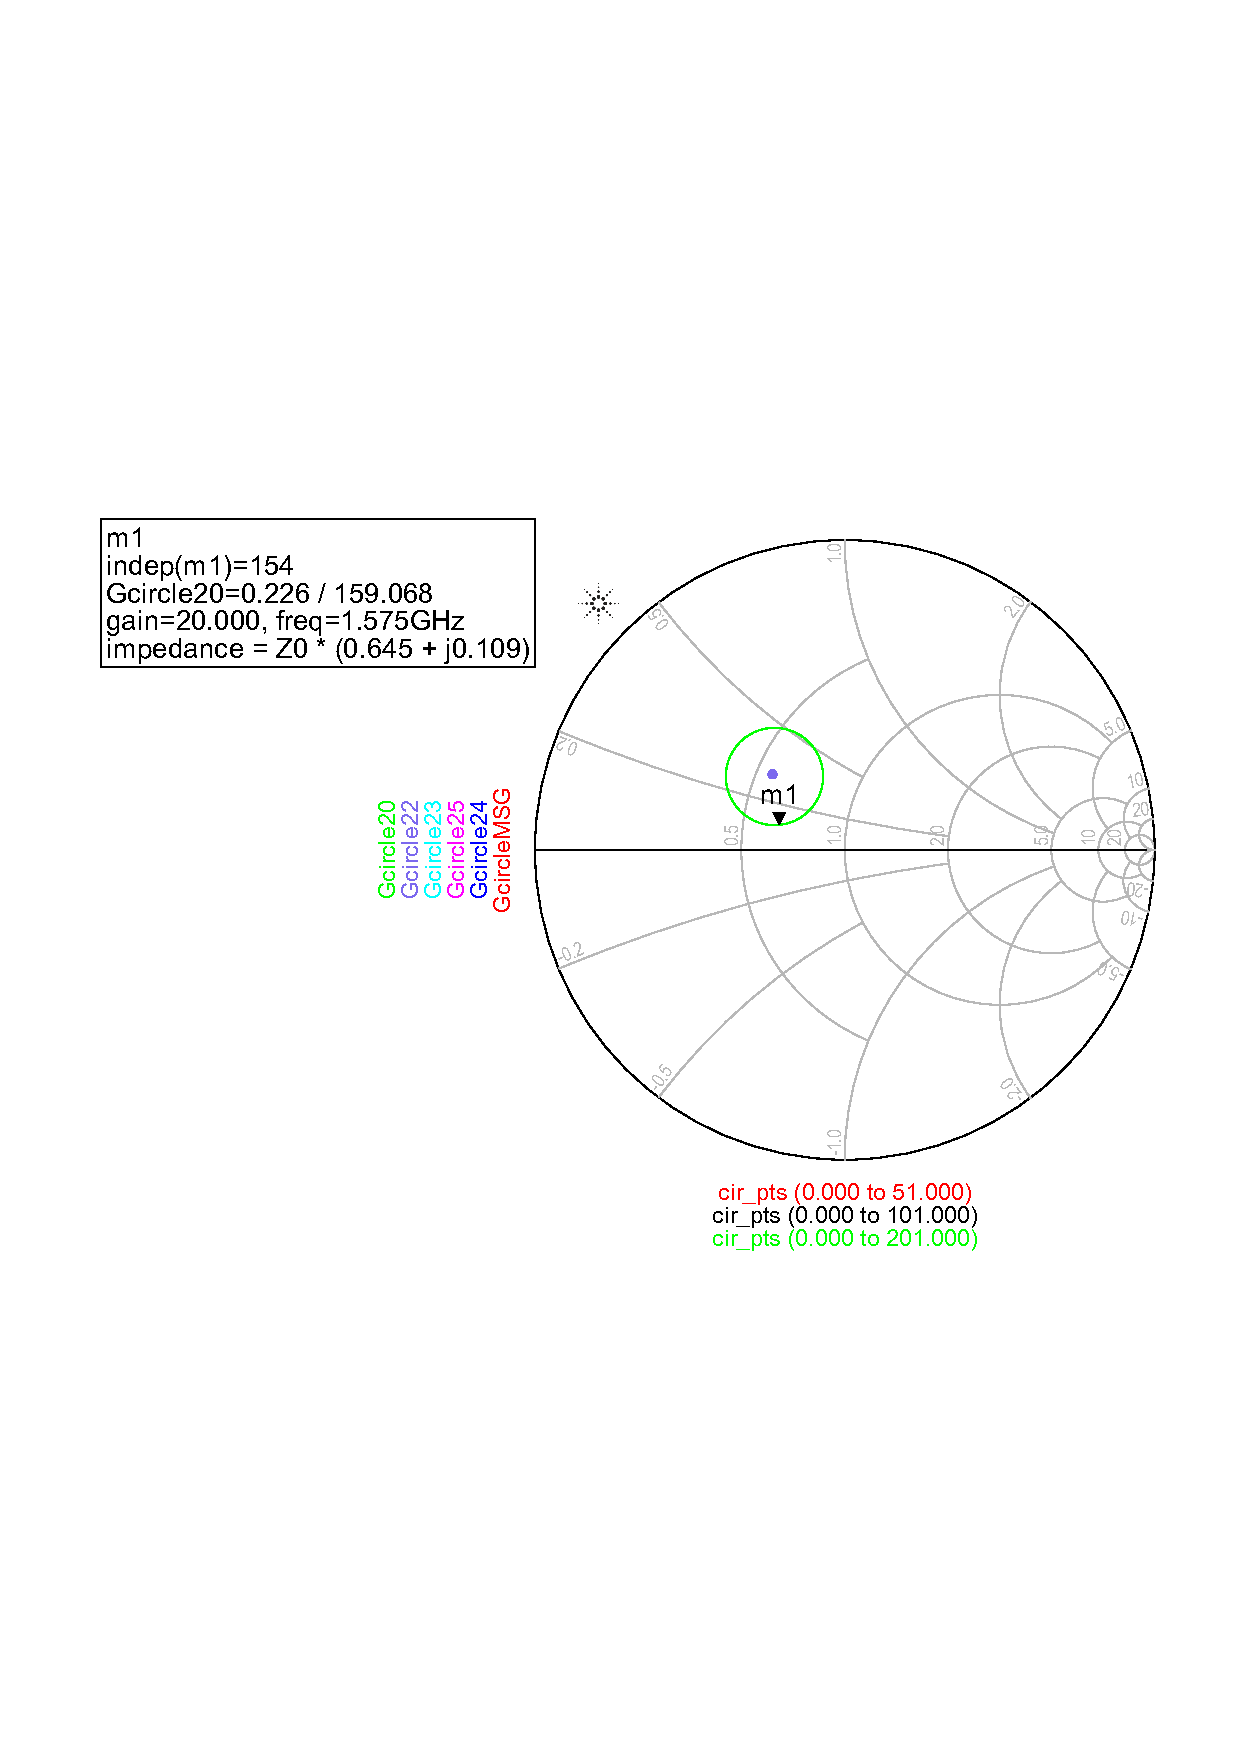
\includegraphics[width=\textwidth]{fig/LNA/LNA_gain_circle.pdf}
			\end{subfigure}
			\begin{subfigure}{0.5\textwidth}
				\centering
				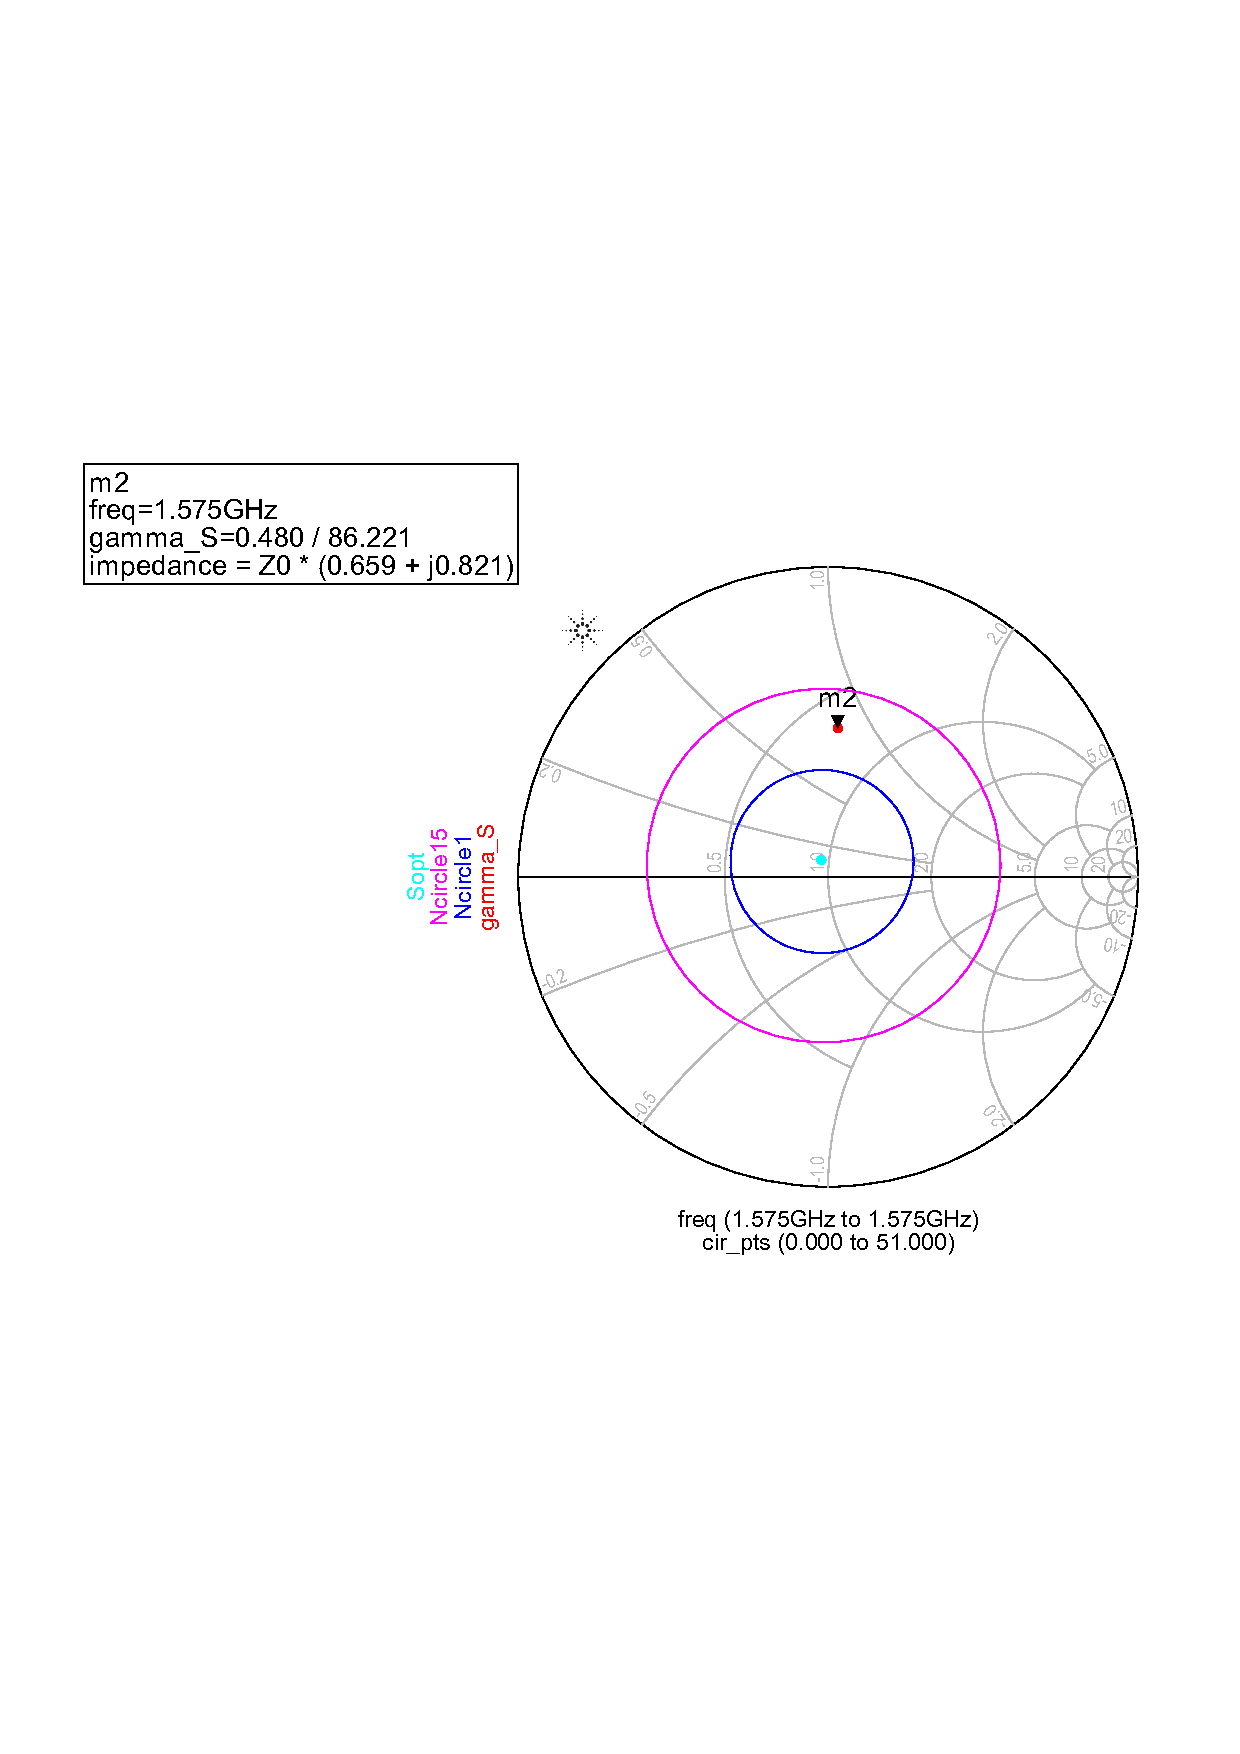
\includegraphics[width=\textwidth]{fig/LNA/LNA_noise_circle.pdf}
			\end{subfigure}
				\caption{Constant Noise and Gain circles for matching}
				\label{fig:lna_circles}
			\end{figure}

			The next step is to replace the ideal base current source by a biasing network. This biasing network will induce negative feedback and thus ensure stability. The voltage drop over the resistor will be $V_{CE} - \SI{0.7}{\volt} = \SI{3.3}{\volt}$ and the current needs to be $\SI{66}{\micro\ampere}$, hence $R = \SI{50}{\kilo\ohm}$. After tuning for best performance, we obtain the circuit shown in Figure \ref{fig:lna_pre_layout}.

			\begin{figure}[H]
				\centering
				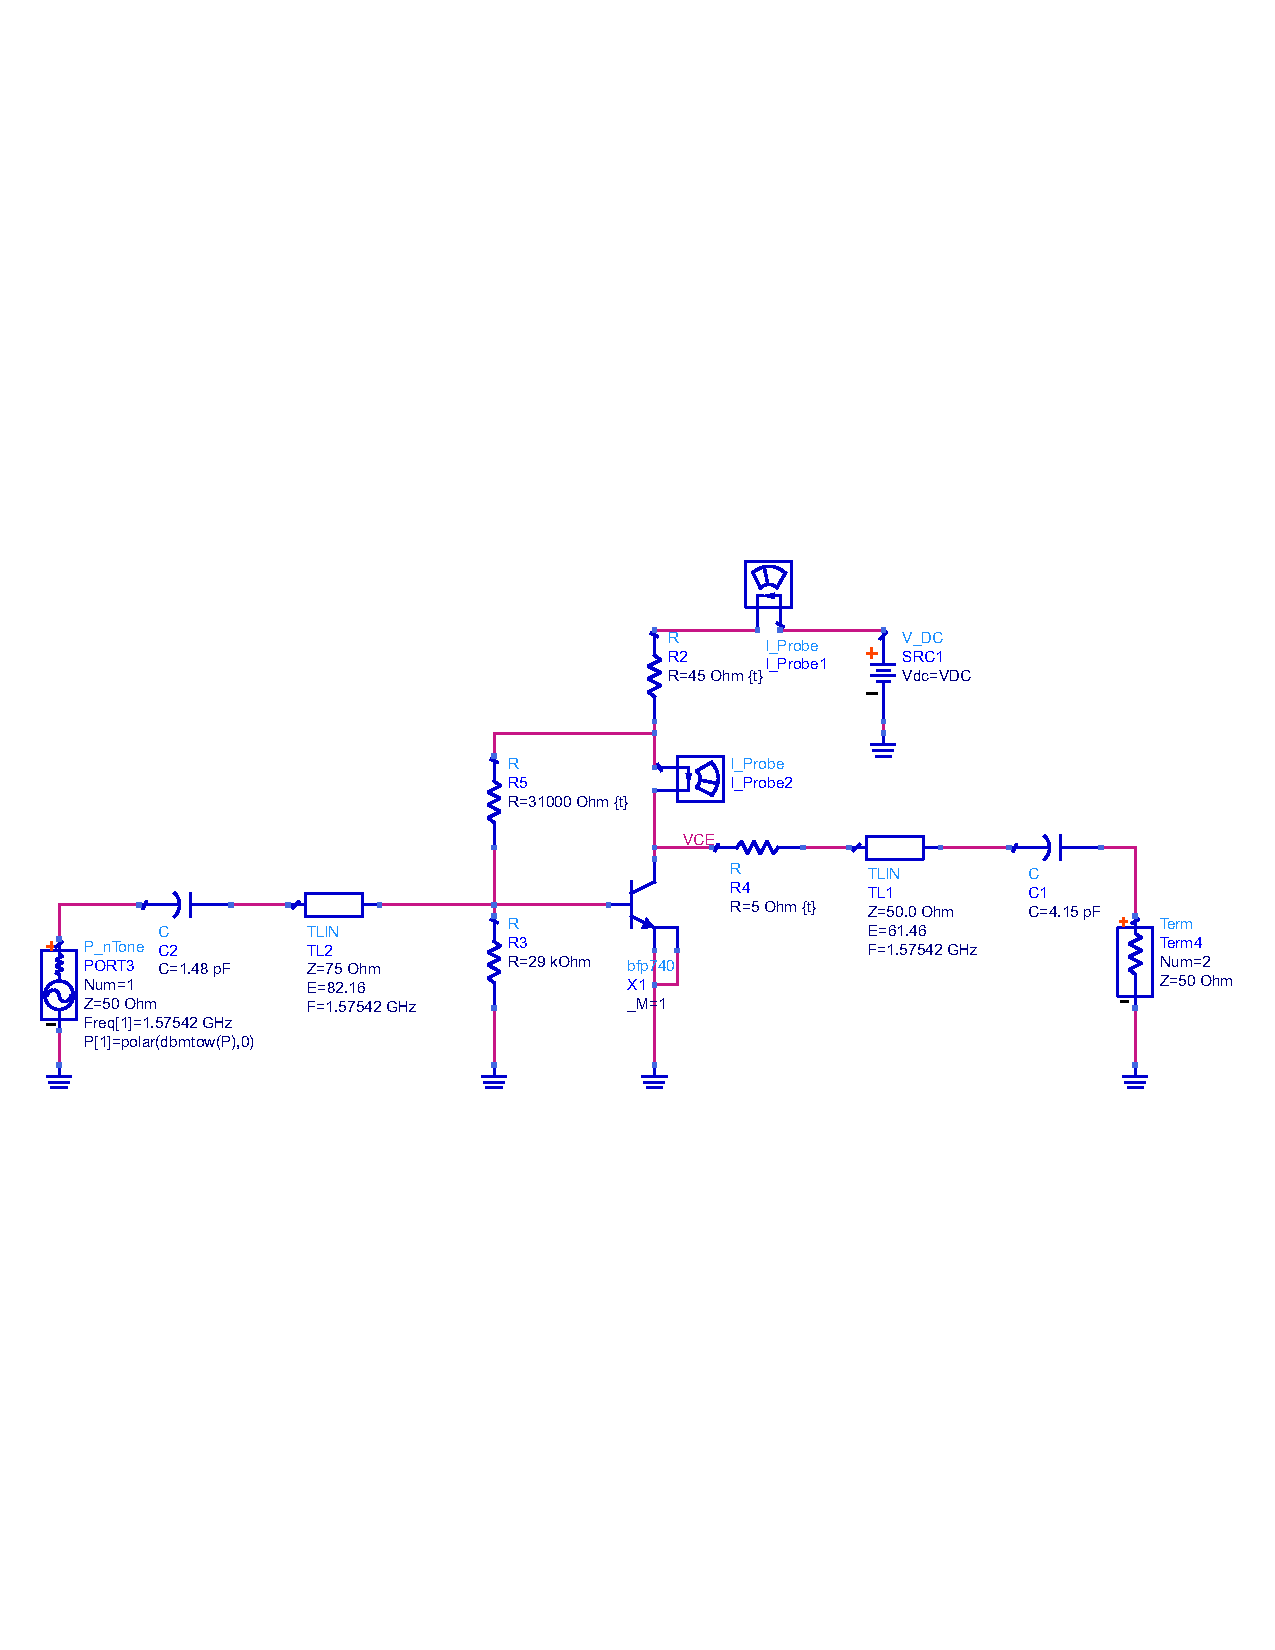
\includegraphics[width=0.8\textwidth]{fig/LNA/LNA_matched.pdf}
			\caption{Realized circuit after matching and biasing}
			\label{fig:lna_pre_layout}
			\end{figure} 

			The Smith Chart in Figure \ref{fig:lna_matching_smith} shows that the input is perfectly matched to $\SI{50}{\ohm}$ after adding the matching networks from Figure \ref{fig:lna_pre_layout}. The output is on purpose mismatched to obtain a NF that is smaller than $\SI{1.5}{\decibel}$ (see \ref{sec:lna_matching}).

			\begin{figure}[H]
			\centering
				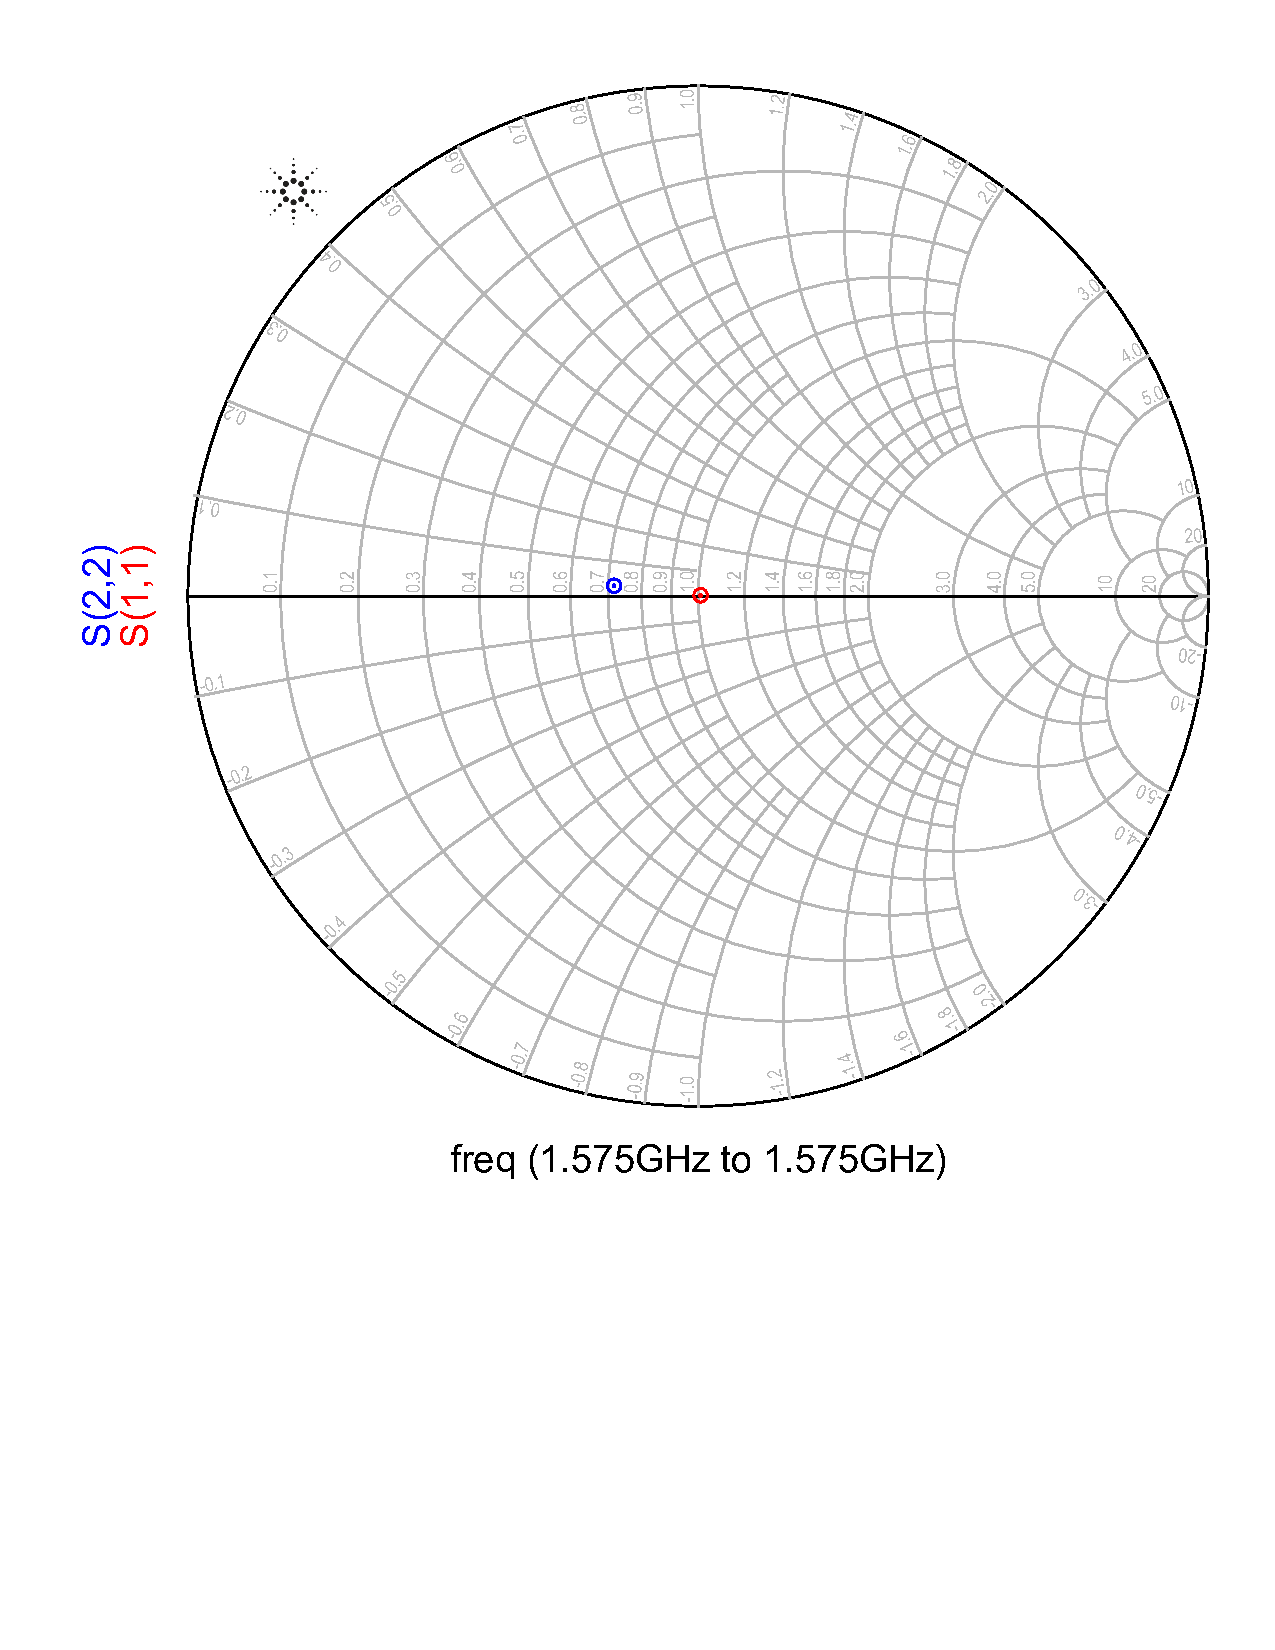
\includegraphics[width=0.5\textwidth]{fig/LNA/matching_smith.pdf}
			\caption{Smith Chart after adding matching network}
			\label{fig:lna_matching_smith}
			\end{figure}

		\subsubsection{Gain and Noise Linearity}

			To obtain the 1dB Compression Point large signal S-parameters need to be simulated. The difference between the simulated gain characteristic and the ideal (linear) gain characteristic is plotted as a function of the input power in Figure \ref{fig:lna_1dbcp}. We see that the 1-dBCP is reached for an input power equal to $\SI{-15.5}{\dbm}$. We also know that the gain of the amplifier is $\SI{20}{\decibel}$, hence we get an output referred 1-dBCP of $\SI{4.5}{\dbm}$ which is within the specifications. To increase the linearity further, we added inductive emittor degeneration with an inductor of $\SI{100}{\pico\henry}$. This will not be a physical component, but the inductance will be present due to the vias to the ground plane. 

			\begin{figure}[H]
			\centering
				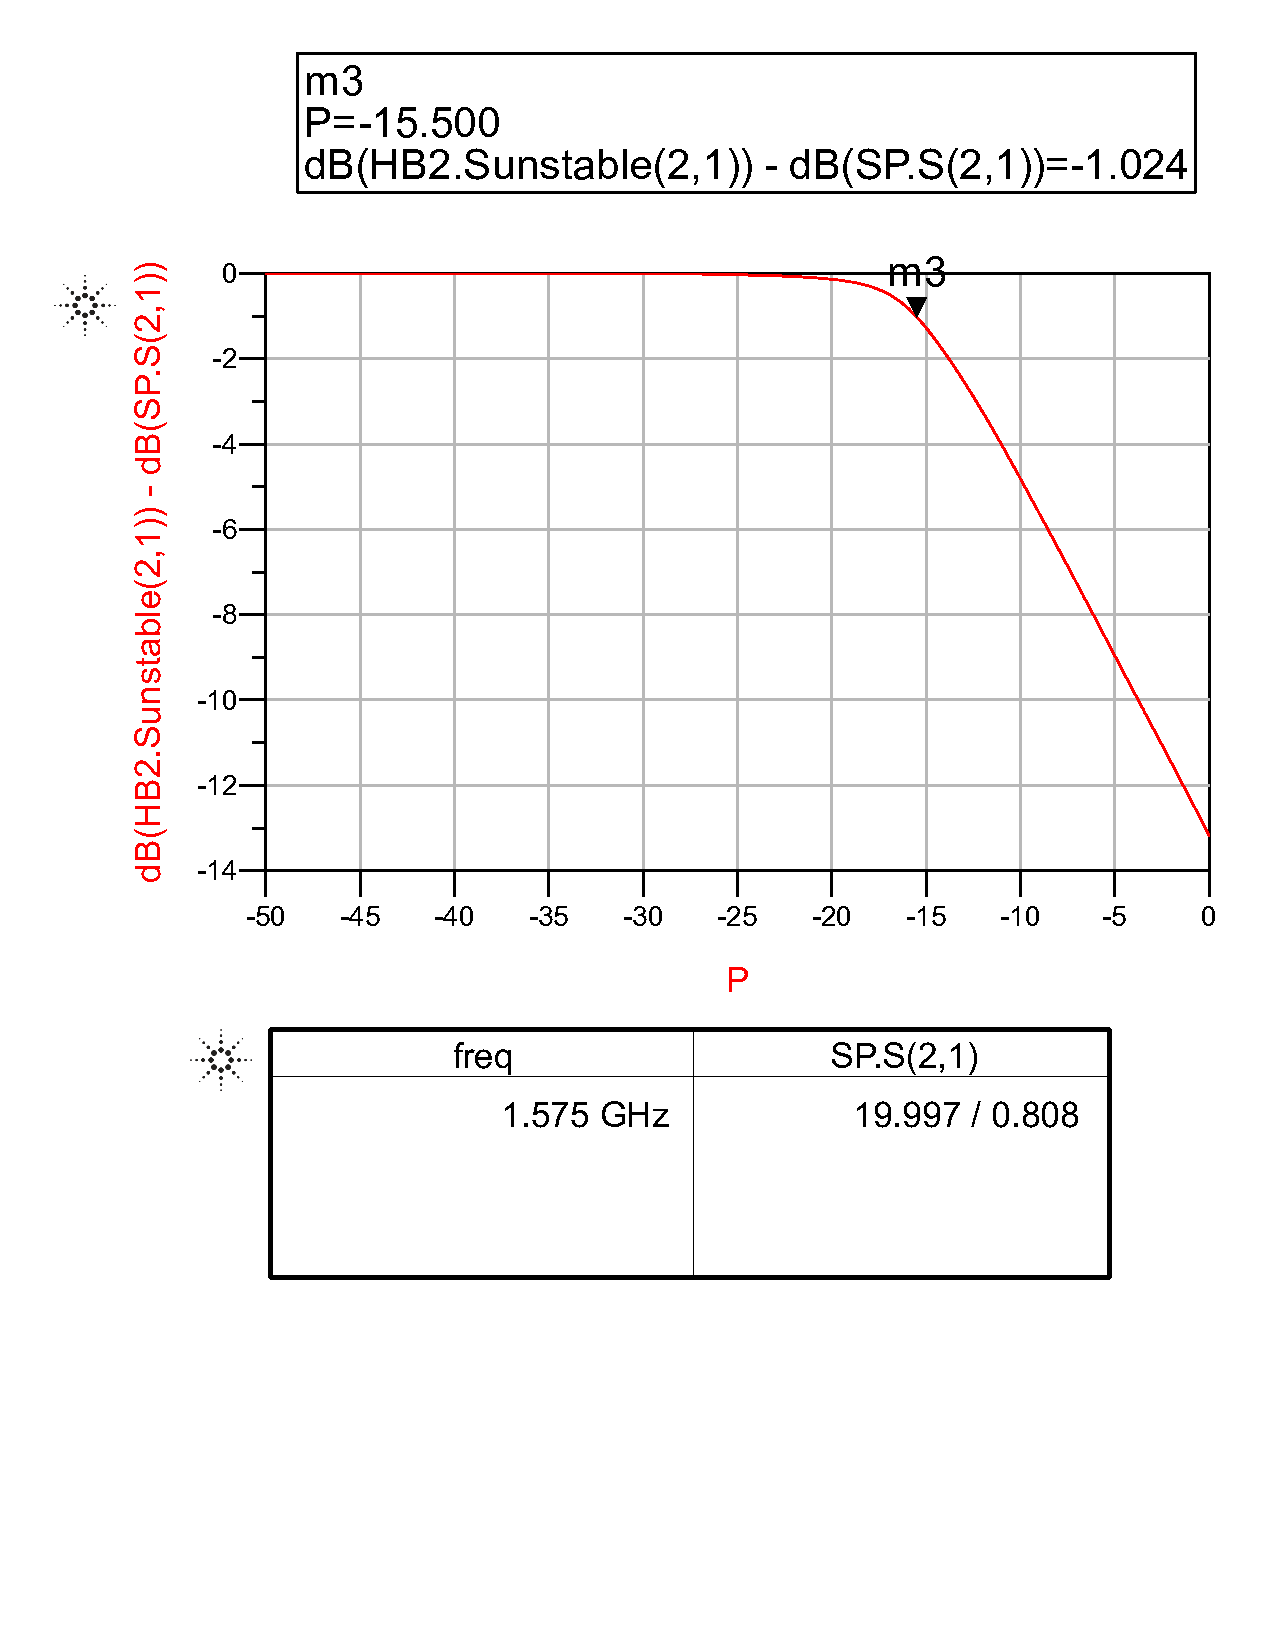
\includegraphics[width=0.5\textwidth]{fig/LNA/compression_point.pdf}
			\caption{Simulated 1 dB Compression Point}
			\label{fig:lna_1dbcp}
			\end{figure}

		\subsubsection{Figure of Merrit}
			We want the LNA to be as linear as possible, but the DC power consumption needs to be kept as low as possible. That's why we will use the ratio $\frac{OIP3}{P_{DC}}$ as a figure of merrit (FOM), with $OIP3$ the Output Referred Third Order Intercept Point and $P_{DC}$ the DC power consumption. The higher the FOM, the higher the linearity of the amplifier and the lower the power consumption. \\

			To calculate OIP3 we perfom a Harmonic Balance simulation in ADS, i.e. we send two tones into the circuit and observe the third order mixing products. Figure \ref{fig:lna_fom} shows these third order products and their output referred intercept point in the table below the figure. 
			
			\begin{figure}[H]
				\centering
				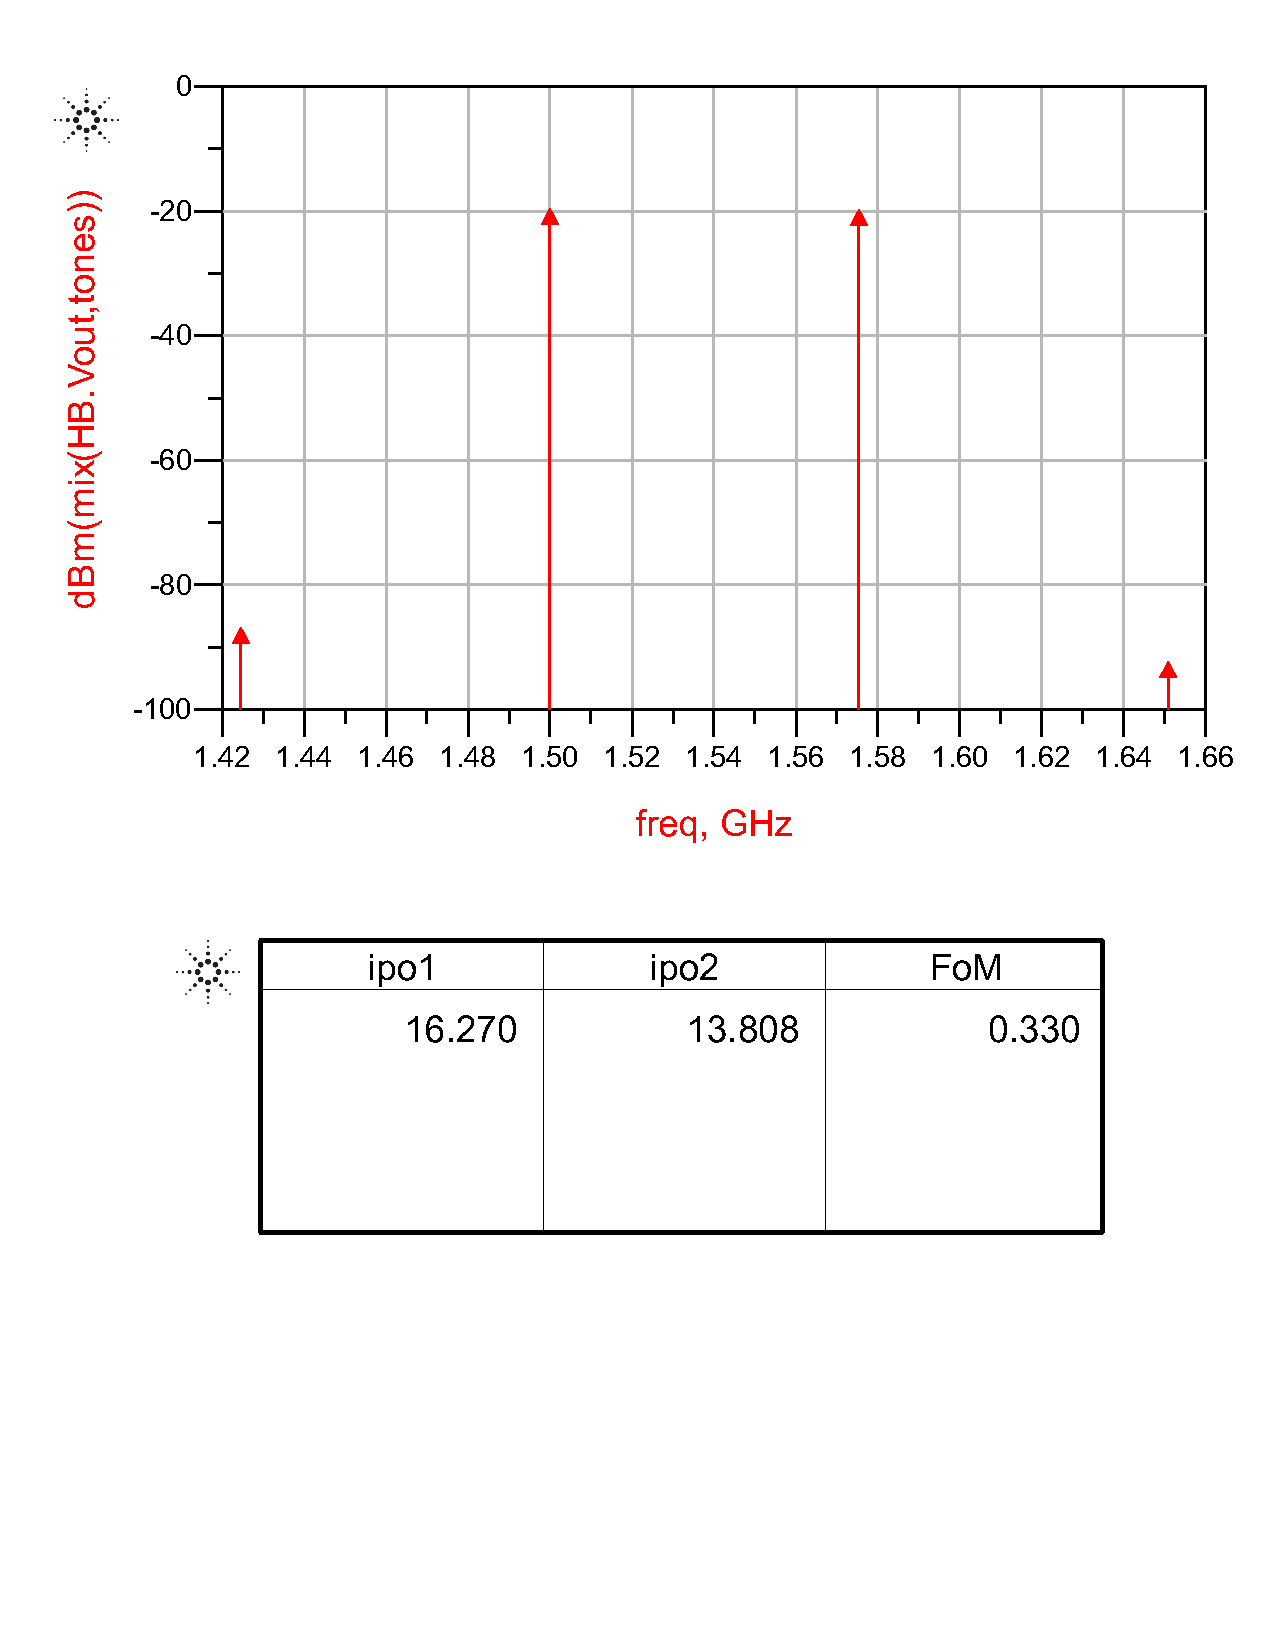
\includegraphics[width=0.5\textwidth]{fig/LNA/fom.pdf}
				\caption{Figure of Merrit}
				\label{fig:lna_fom}
			\end{figure}

		\subsubsection{Summary}
			Table \ref{tab:lna_summ} gives an overview of the simulated design parameters compared with the specifications. It can be seen that in this stage of the design all specifications are still met.  

			\begin{table}[H]
			\centering
			\begin{tabular}{|l|r|r|}
				\hline
				 & \textbf{Realized} & \textbf{Specs} \\
				\hline
				\textbf{SS Gain} & 20 dB & $>$ 16 dB \\
				\hline
				\textbf{NF} & 1.196 dB & $\leq$ 1.5 dB \\
				\hline
				\textbf{Output ref. 1dBCP} & 4.5 dBm & $>$ 3 dBm \\
				\hline
				\textbf{FOM} & 0.33 & n/a \\
				\hline
			\end{tabular}
			\caption{Summarizing achieved specs}
			\label{tab:lna_summ}
			\end{table}

		
	\subsection{Filter}

\section{Layout}
	\subsection{LNA}
		\subsubsection{Generation of Layout}
			Before generating a layout for the designed LNA circuit, the schematic is made layout friendly. This means the nets in the schematic are replaced by transmission line segments with appropriate impedance, pads for the discrete components are added and discontinuities in microstrip line thickness are modeled in the schematic. After generating a layout from the schematic ground planes are added and vias are placed to connect to the underlying ground plane. A plane for the DC supply voltage is added as well and is placed close to the ground plane for decoupling of the supply voltage, i.e. the small gap acts as a decoupling capacitance. The resulting layout is shown in Figure \ref{fig:lna_layout}. All traces have a width according to an impedance of $\SI{50}{\ohm}$ except for the transmission line in the matching network at the input, which is $\SI{75}{\ohm}$ to reduce the length of the line, and the trace between collector and base as only DC-current flows there. 

			\begin{figure}[H]
			\centering
				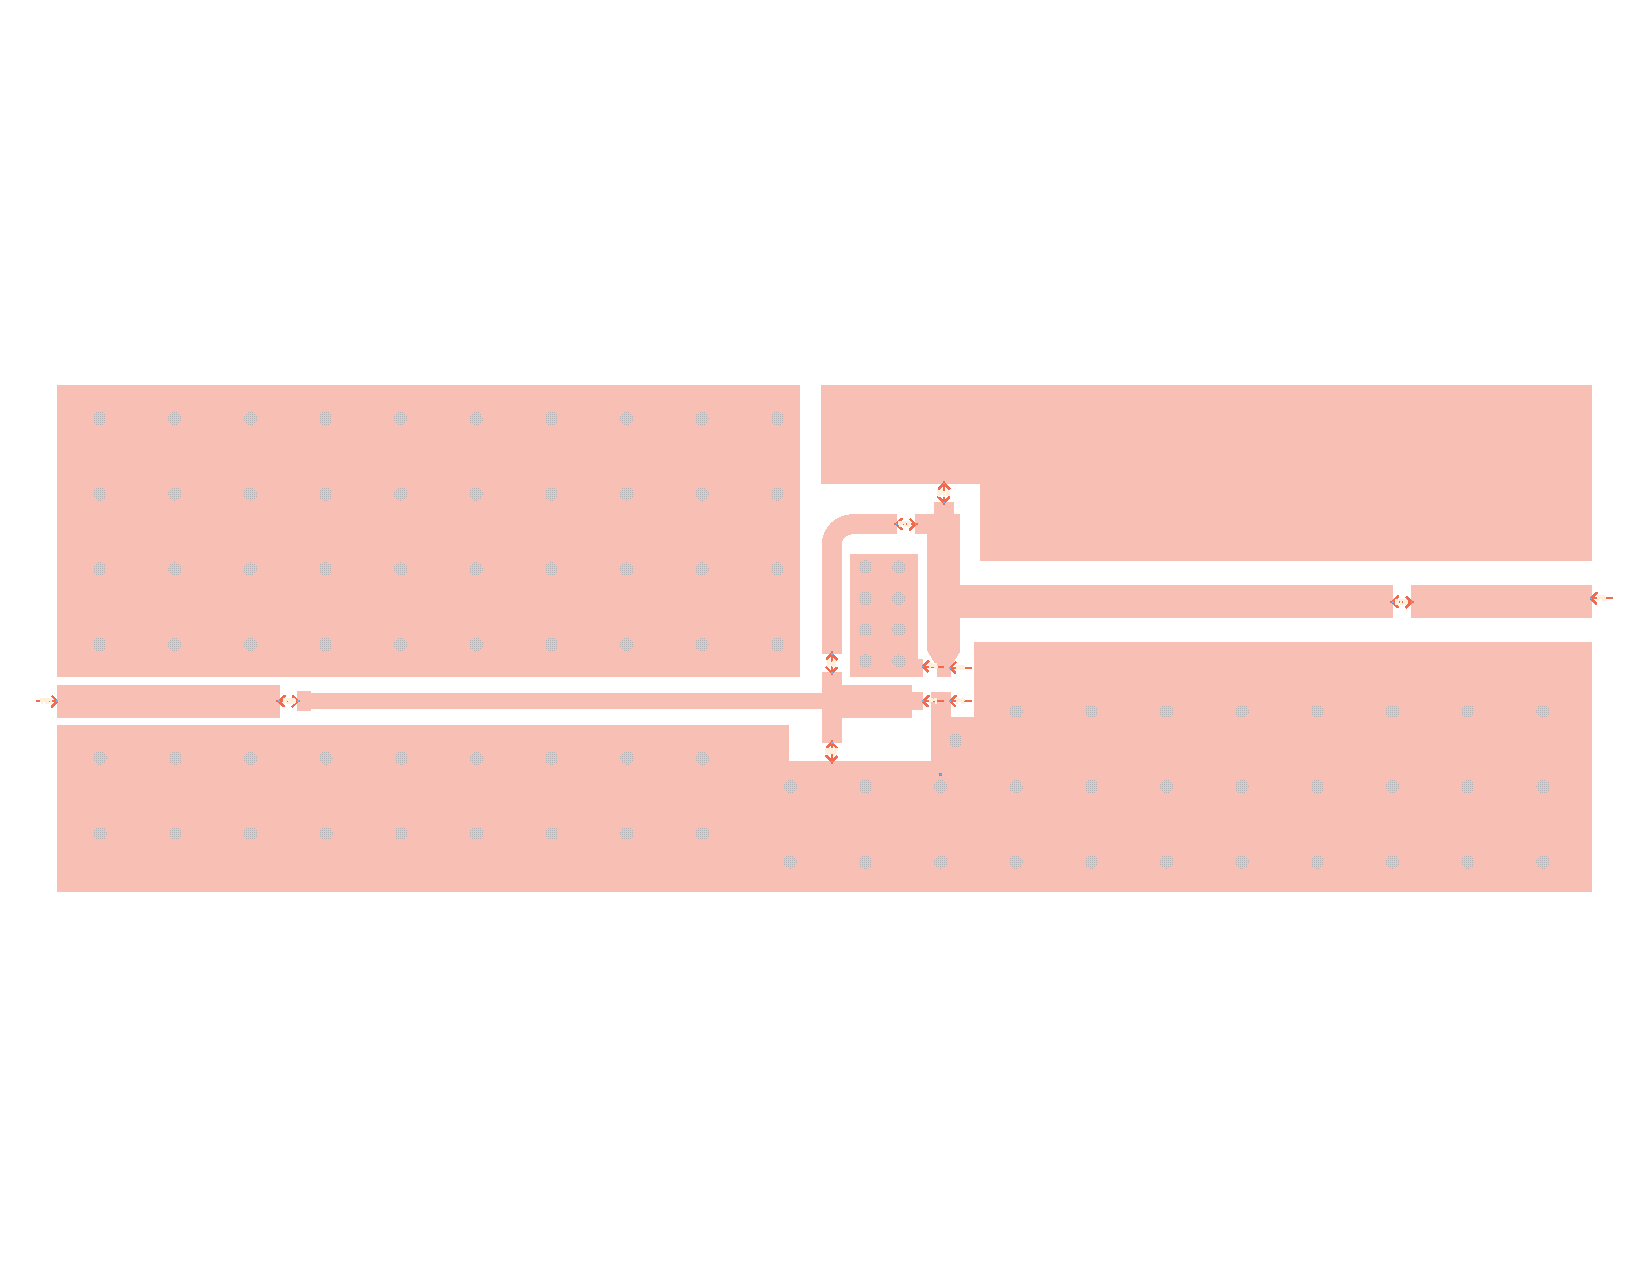
\includegraphics[width=\textwidth]{fig/LNA/LNA_layout.pdf}
				\caption{Generated layout with added ground and source planes}
				\label{fig:lna_layout}
			\end{figure}

		\subsubsection{EM-model Simulations}
			In this step of the design Momentum (full wave) simulations are performed on the drawn layout and an EM-model is generated. This model contains information on transmission line effects, radiation losses, copper losses etc. and can be used to conduct further simulations to better predict the performance of the fabricated device and investigate the differences with the schematic. \\

			The Smith Chart in Figure \ref{fig:lna_smith_post} shows that with inclusion of the EM-model there is a very small mismatch at the input, but the $S_{11}$ is $\SI{-22}{\decibel}$ which is very much acceptable.

			\begin{figure}[H]
			\centering
				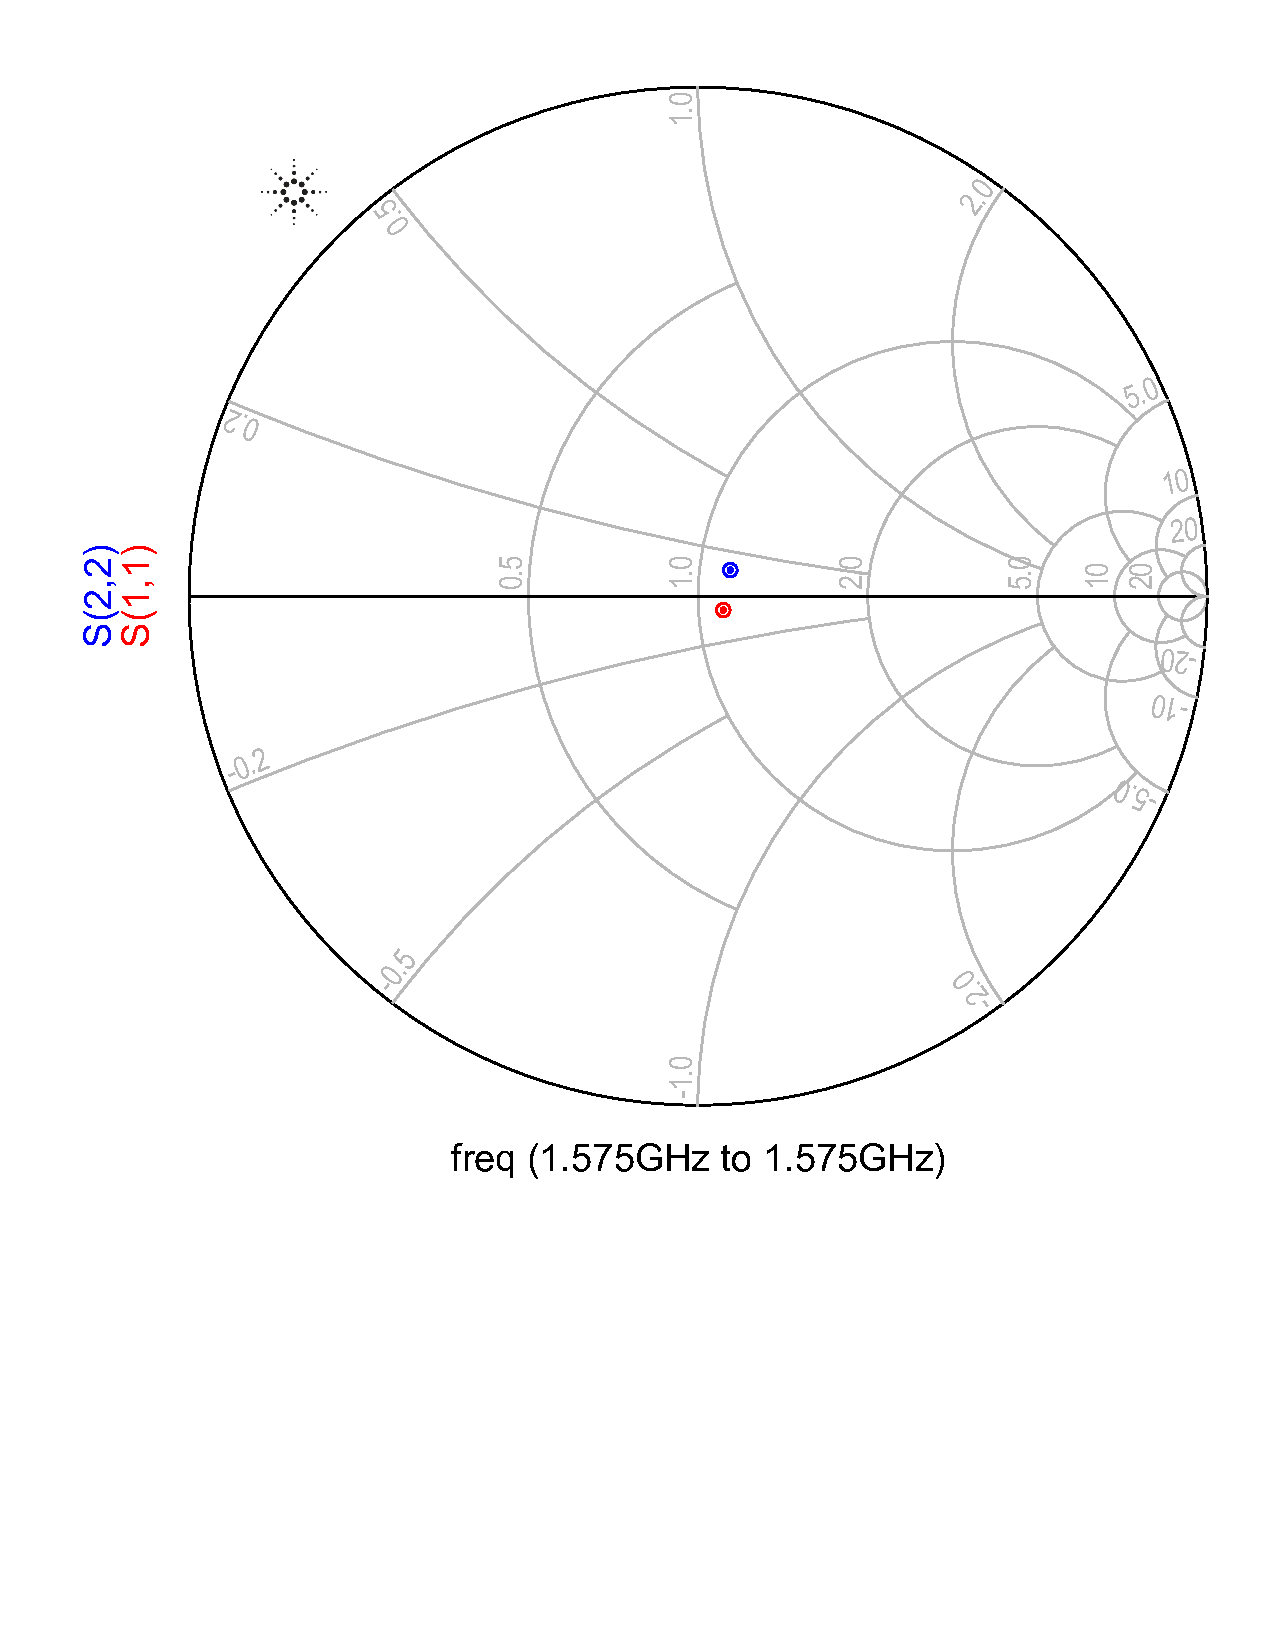
\includegraphics[width=0.5\textwidth]{fig/LNA/matching_post.pdf}
			\caption{Smith Chart with EM-model}
			\label{fig:lna_smith_post}
			\end{figure}

			If we look at the 1-dBCP in Figure \ref{fig:lna_1db_post} we see that the input referred 1-dBCP has increased with $\SI{1}{\dbm}$, but the gain has dropped with approximately the same amount. We get an output referred 1-dBCP of $\SI{4.37}{\dbm}$, which is very close to the value obtained with the schematic ($\SI{4.5}{\dbm}$). 

			\begin{figure}[H]
			\centering
				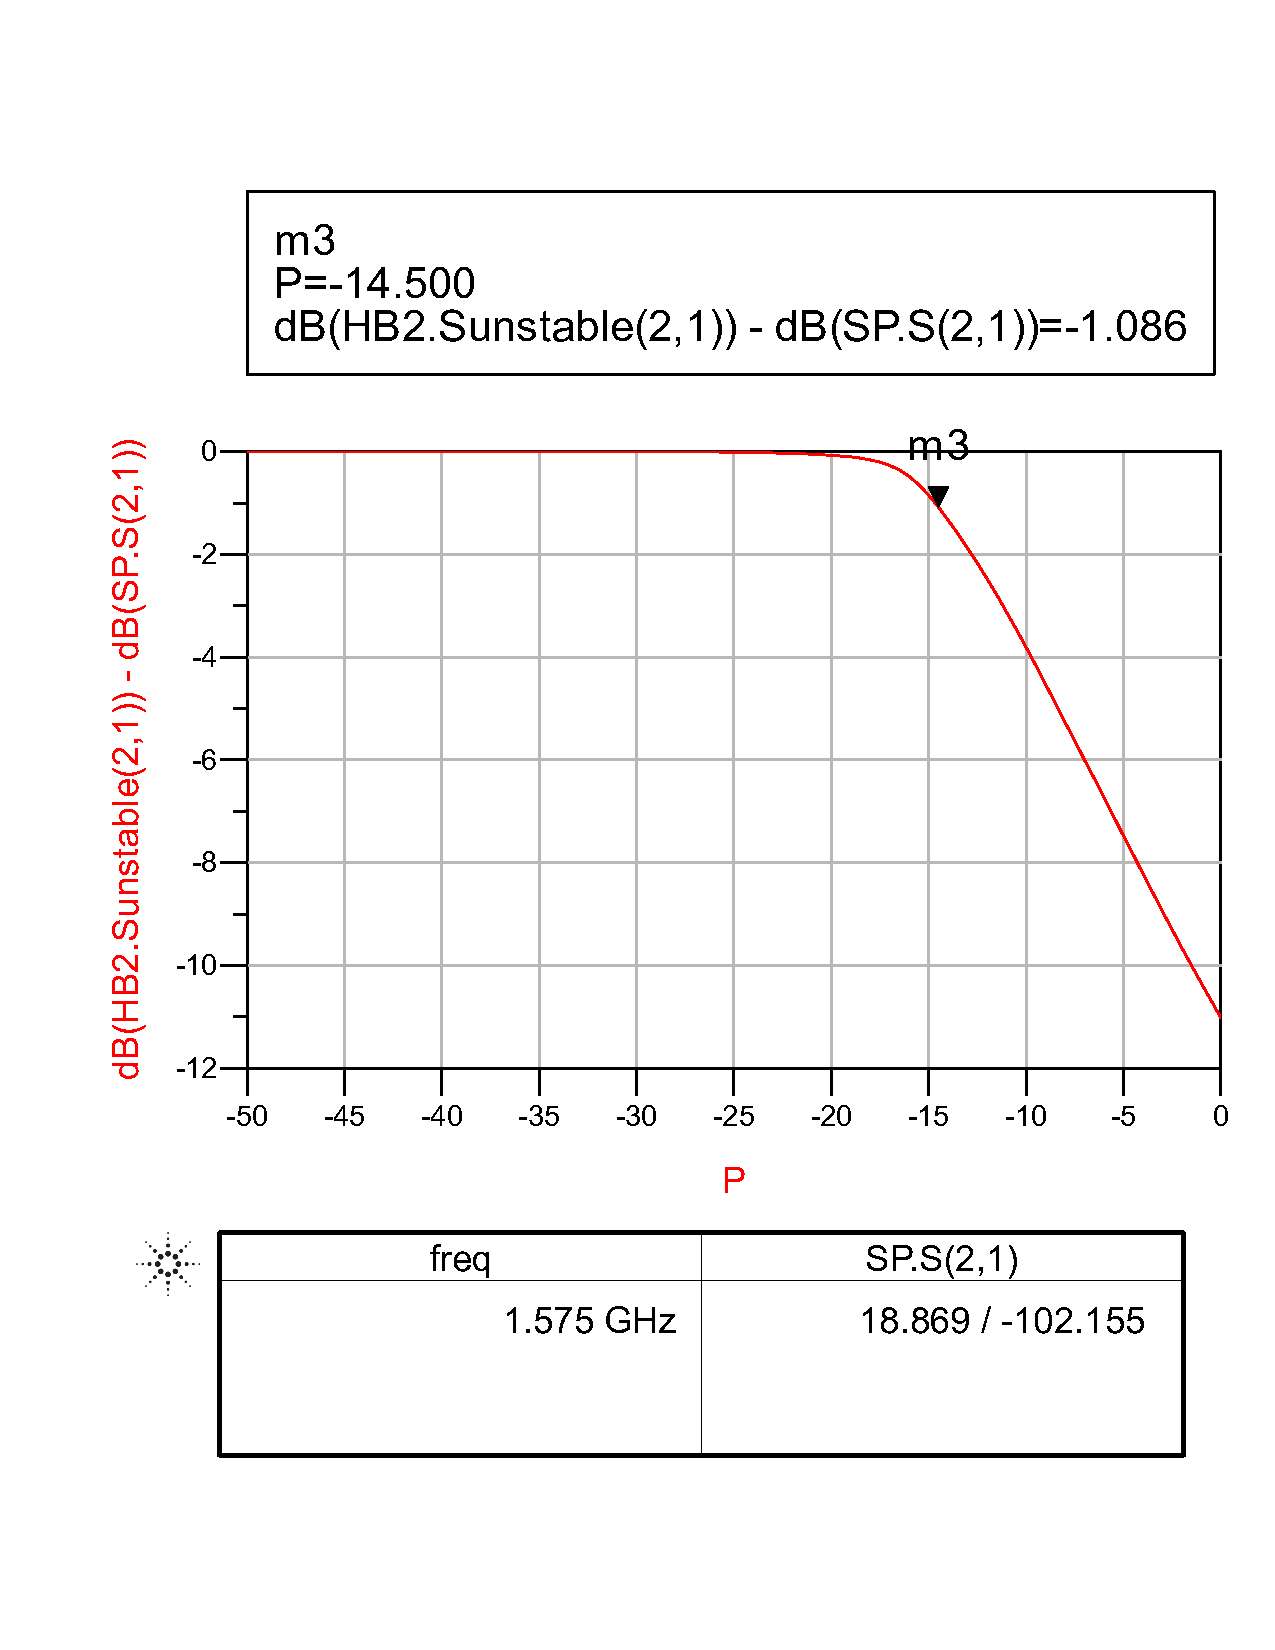
\includegraphics[width=0.5\textwidth]{fig/LNA/compression_post.pdf}
			\caption{1 dB Compression Point with EM-model}
			\label{fig:lna_1db_post}
			\end{figure}

		\subsubsection{Summary}

			\begin{table}[H]
			\centering
			\begin{tabular}{|l|r|r|r|}
				\hline
				 &  \textbf{EM-model} &  \textbf{Schematic} & \textbf{Specs} \\
				\hline
				\textbf{SS Gain} & 18.87 dB &  20 dB & $>$ 16 dB \\
				\hline
				\textbf{NF} & 1.412 dB & 1.196 dB & $\leq$ 1.5 dB \\
				\hline
				\textbf{Output ref. 1dBCP} & 4.37 dBm & 4.5 dBm & $>$ 3 dBm \\
				\hline
				\textbf{FOM} & 0.503 & 0.33 & n/a \\
				\hline
			\end{tabular}
			\caption{Summarizing achieved specs after EM-model simulation}
			\label{tab:lna_em_summ}
			\end{table}


	\subsection{Filter}
\section{Results}
	\subsection{LNA}

	\subsection{Filter}
\section{Conclusion}

\section{Further improvements}

\bibliographystyle{plain}
\bibliography{bookref}
\end{document}